\documentclass{article}
\usepackage{fullpage}
\usepackage{graphicx,xcolor}
\usepackage{url}
\usepackage{amsmath}

\begin{document}

\begin{titlepage}
\begin{center}
%\large
\sffamily


\null\vspace{2cm}
{\huge PCL Toyota Code Sprint 2.0 - Superquadrics} \\[24pt] 
\textcolor{gray}{{\\ Alexandru - Eugen Ichim}}
    
\vfill

\begin{tabular} {cc}
\hspace{1cm}
\parbox{0.4\textwidth}{
\includegraphics[width=6cm]{figures/logos}}
\hspace{4cm}
&
\parbox{0.7\textwidth}{%
	Open Perception Inc. \\ \\ \\
%
\small
Supervised by:\\[4pt]
%
    Dr. Joseph Djugash\\
    Dr. Radu B. Rusu\\[12pt]
%
2013}
\end{tabular}
\end{center}
\vspace{2cm}
\end{titlepage}


%%%%%%%%%%%%%%%%%%%%%%%%%%%%%%%%%%%%%%%%%%%%%%%%%%%%%%%%%%%%
%%%%%%%%%%%%%%%%%%%%%%%%%%%%%%%%%%%%%%%%%%%%%%%%%%%%%%%%%%%%

\tableofcontents
\newpage

\section {Introduction}

\subsection {Code Sprint}
A code sprint is an accelerated research and development program, inspired by the Google Summer of Code model, and organised within the Point Cloud Library project by the host foundation, Open Perception Inc. PCL developers are paired with senior researchers and engineers from various institutions for extended R\&D work with financial backup.

The first code sprint in which Toyota got involved was done in 2012, and one of the projects was that of implementing novel smoothing algorithms \cite{tocs_final_report}.

\subsection {Target}
The target of the current code sprint is that of analysing the possibilities of using superquadric object representation in robotics computer vision tasks such as object detection. 

The structure of this report is as follows. In this section we continue by introducing the concept of superquadrics and some mathematical background, as well as sources of datasets we have used for development. Next, in section \ref{sec:sampling}, we look into techniques for sampling the superquadric equation in order to get point clouds and meshes. Section \ref{sec:fitting} shows the approaches we implemented for fitting superquadric objects into point clouds, with the extension of fully describing a point set as a collection of non-overlapping superquadrics. We then look into how to efficiently find objects for which we now the parametric representation in a new point cloud - section \ref{sec:detection}. Finally, we show a complete demo using an RGB-D sensor in Section \ref{sec:tabletop_demo} and conclude with section \ref{sec:conclusion}.


\subsection {Superquadrics}

\subsubsection*{History}
The concept of superquadrics was first introduced in the Computer Graphics community in \cite{1673799}, as a means of versatile parametric object modelling. The mathematical details have been extended in the work of Jakli\v{c} et al. \cite{SQ_2000}. Just like quadrics, superquadrics can be split into superellipsoids, superhyperboloids of one piece, superhyperboloids of two pieces and supertoroids, but for the purpose of our work, we only focused on superellipsoids (see Figure \ref{fig:superquadric_family}).

%%% TODO - figure with superellipsoid, toroid, and hyperboloids of one and two sheets
\begin{figure}
\centering
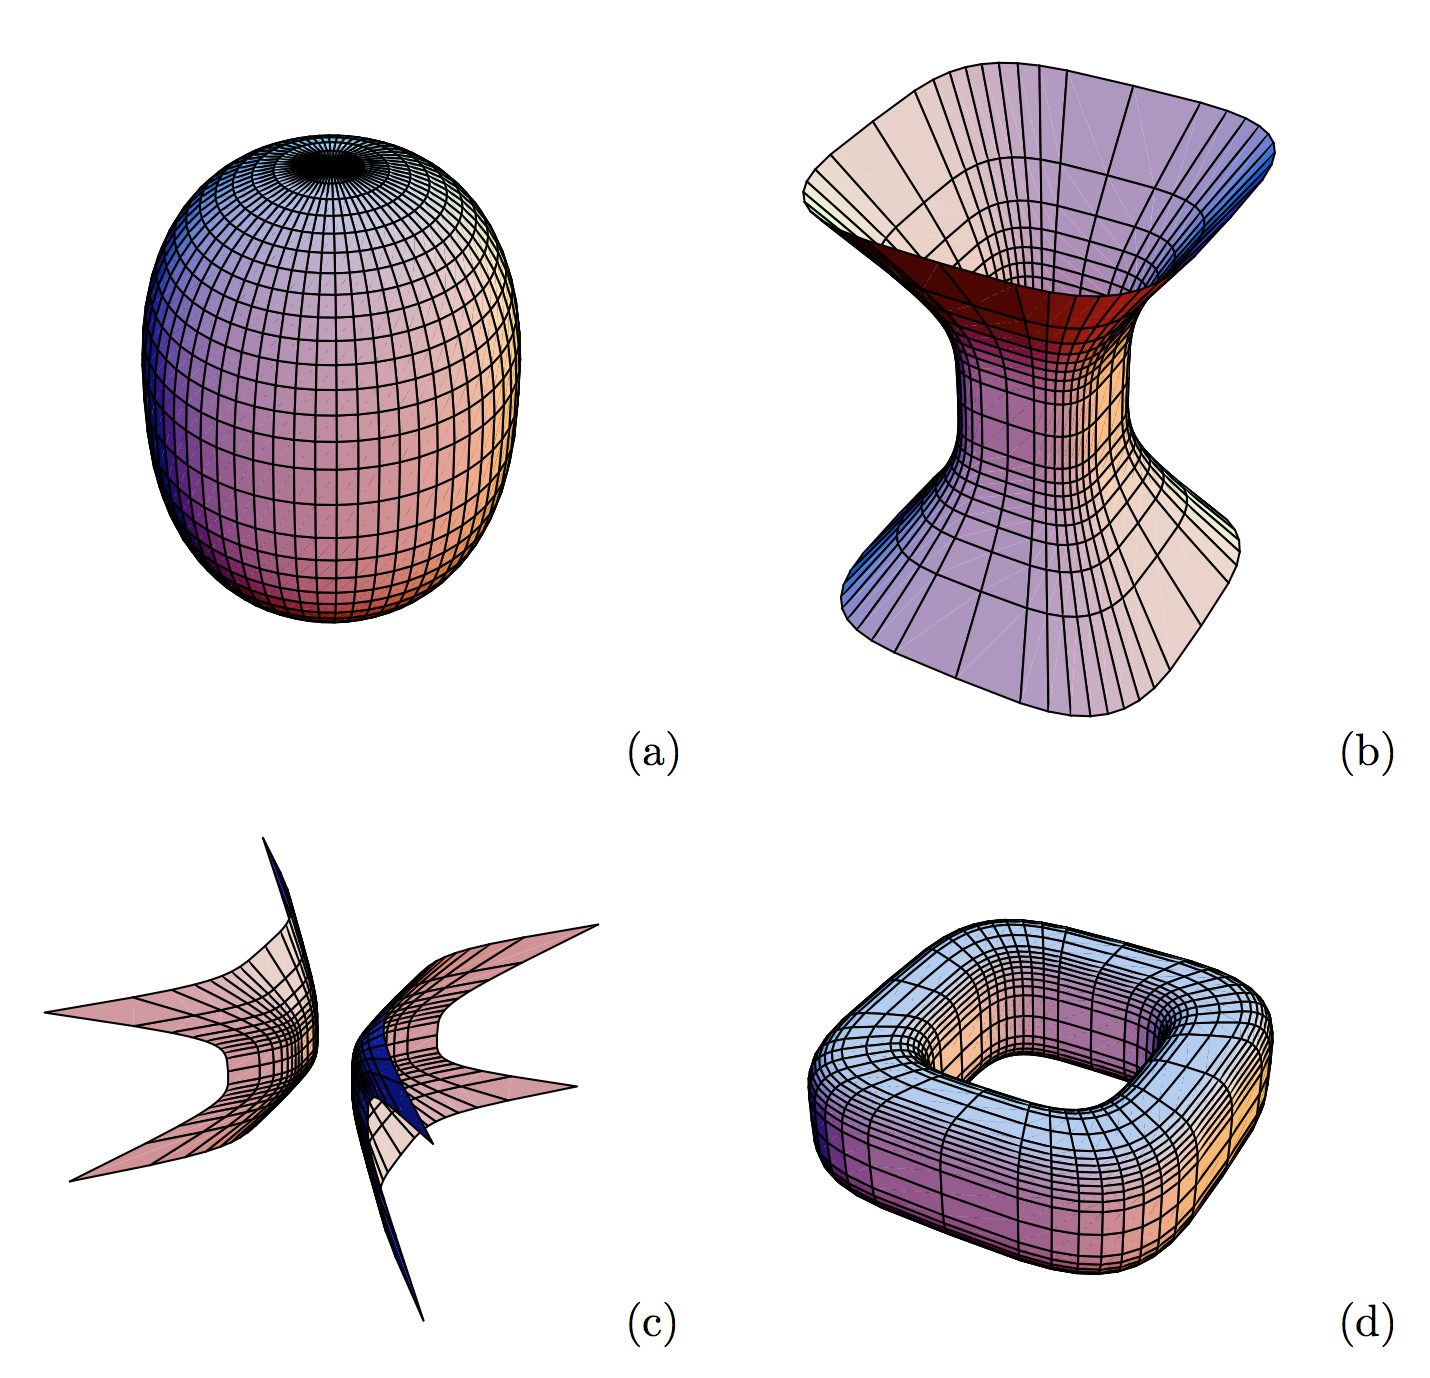
\includegraphics[width=0.5\columnwidth]{figures/superquadric_family}
\caption{Family of superquadrics: (a) superellipsoid, (b) superhyperboloid of one sheet, (c) superhyperboloid of two sheets, (d) supertoroid}
\label{fig:superquadric_family}
\end{figure}

\subsubsection*{Mathematical Definition}
They are created from two two-dimensional curves (a horizontal and a vertical curve) that form a three-dimensional surface under spherical product. For example, a unit sphere is created as the spherical product of a half circle in the plane orthogonal to $(x, y)$ is crossed with the full circle in the $(x, y)$ plane.

\begin{equation}
m (\eta) = \begin{pmatrix} \cos {\eta} \\ \sin{\eta} \end{pmatrix}
\end{equation}

\begin{equation}
h(\omega) = \begin{pmatrix} \cos {\omega} \\ \sin {\omega} \end{pmatrix}
\end{equation}

with $\eta \in [-\pi/2, \pi/2]$ and $\omega \in [-\pi, \pi)$.

The sphere becomes:

\begin{equation}
r (\eta, \omega) = m (\eta) \oplus h (\omega) = \begin{pmatrix} \cos{\eta} \cos{\omega} \\ \cos{\eta} \sin{\omega} \\ \sin{\omega} \end{pmatrix}
\end{equation}

A superellipsoid can be obtained by the spherical product of two superellipses of the form:

\begin{equation}
\left(\frac{x}{a}\right)^{\frac{2}{\epsilon}} + \left(\frac{y}{b}\right)^{\frac{2}{\epsilon}} = 1
\end{equation}

\begin{equation}
s(\theta) = \begin{pmatrix} a \cos^\epsilon{\theta} \\ b \sin^\epsilon {\theta} \end{pmatrix} \textnormal{, with } \theta \in [-\pi, \pi]
\end{equation}

\begin{equation}
r (\eta, \omega) = s_1 (\eta) \oplus s_2 (\omega) = \begin{pmatrix} \cos^{\epsilon_1} {\eta} \\ a_3 \sin^{\epsilon_1} {\eta} \end{pmatrix} \oplus \begin{pmatrix} a_1 \cos^{\epsilon_2} {\omega} \\ a_2 \sin^{\epsilon_2} {\omega} \end{pmatrix} = \begin{pmatrix} a_1 \cos^{\epsilon_1} {\eta} \cos^{\epsilon_2} {\omega} \\ a_2 \cos^{\epsilon_1} {\eta} \sin^{\epsilon_2} {\omega} \\ a_3 \sin^{\epsilon_1}{\eta}\end{pmatrix} \textnormal{, with } \eta \in [-\pi/2, \pi/2], \omega \in [-\pi, \pi)
\end{equation}

The five parameters of a superellipse are as follows:

\begin{itemize}
	\item {\textbf{$a_1$, $a_2$, $a_3$} - scaling factors along the three axes}
	\item {\textbf{$\epsilon_1$} - the shape of the superellipsoid cross section in a plane orthogonal to the $(x, y)$ plane and containing the $z$-axis}
	\item {\textbf{$\epsilon_2$} - the shape of the superellipsoid cross section parallel to the $(x, y)$ plane}	
\end{itemize}

% TODO Generate superellipsoids with various parameters: vary a,b,c, bigger e1, bigger e2 - 7 figures in total

The implicit equation of a superellipsoid is thus:

\begin{equation}
\left(\left(\frac{x}{a_1}\right)^{\frac{2}{\epsilon_2}} + \left(\frac{y}{a_2}\right)^{\frac{2}{\epsilon_2}}\right)^{\frac{\epsilon_2}{\epsilon_1}} + \left(\frac{z}{a_3}\right)^{\frac{2}{\epsilon_1}} =1
\end{equation}

Because of the inside-outside functions that describe superquadrics, they can be easily manipulated by means of solid boolean operations such as union, intersection and subtraction.

\subsubsection*{Numerical Issues}
There are some issues we need to take into consideration when writing code that involves the usage of superquadrics. All the powers in the implicit function are of the form $2p$: $2/\epsilon_1$, $2/\epsilon_2$, and we compute them in the order $x^{(2p)}=(x^2)^p$ so that they are always positive. In the case of the explicit function, all the powers are actually signed power functions, and are treated as follows:

\begin{equation}
x^p = sgn(x) |x|^p = \left\{
	\begin{array}{ll}
		|x|^p  & \textnormal{if } x \geq 0 \\
		-|x|^p & \textnormal{if } x < 0
	\end{array}
\right.
\end{equation}


Because of the limitation of the range of real numbers a 64-bit system can compute within, we need to clamp the $\epsilon_1$ and $\epsilon_2$ parameters in the interval $(0.1, 1.9)$. Values beyond this range do not introduce a lot more expressiveness to the objects, but creates numerical problems as $\frac{\epsilon_2}{\epsilon_1}$ becomes very large.

\subsection {Datasets}
For the purpose of this work, we gathered data from multiple sources:

\begin{itemize}
	\item{\textbf{Created manually}}
		\begin{figure}[h]
		\centering
		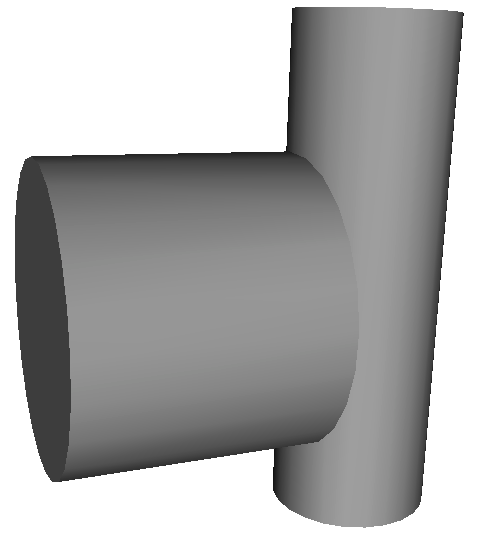
\includegraphics[width=0.2\columnwidth]{figures/2_components}
		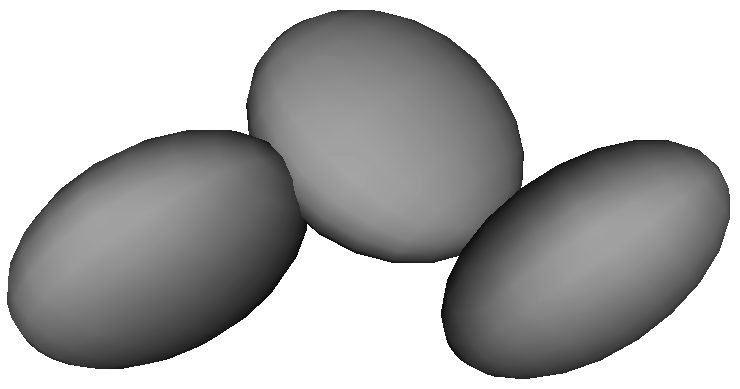
\includegraphics[width=0.3\columnwidth]{figures/3_components}
		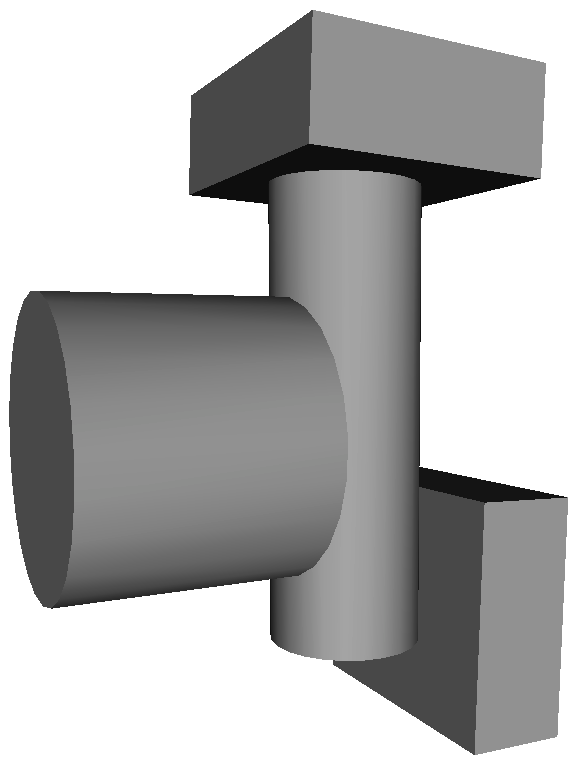
\includegraphics[width=0.2\columnwidth]{figures/4_components}
		\end{figure}

	\item{\textbf{Trimble 3D Warehouse}}
		\begin{figure}[h]
		\centering
		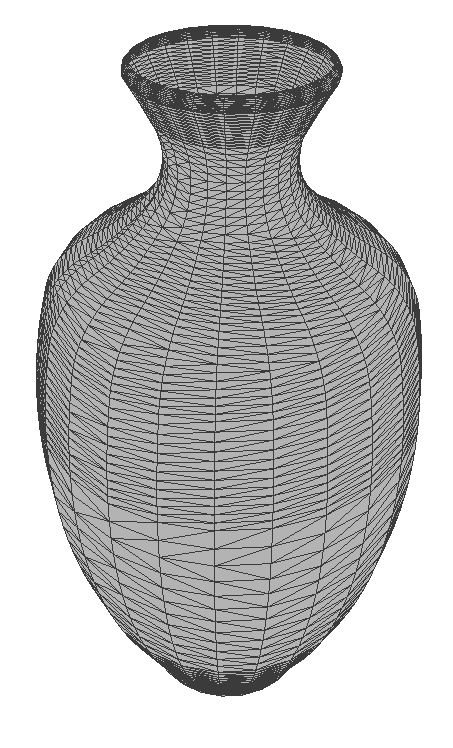
\includegraphics[width=0.2\columnwidth]{figures/vase_1}
		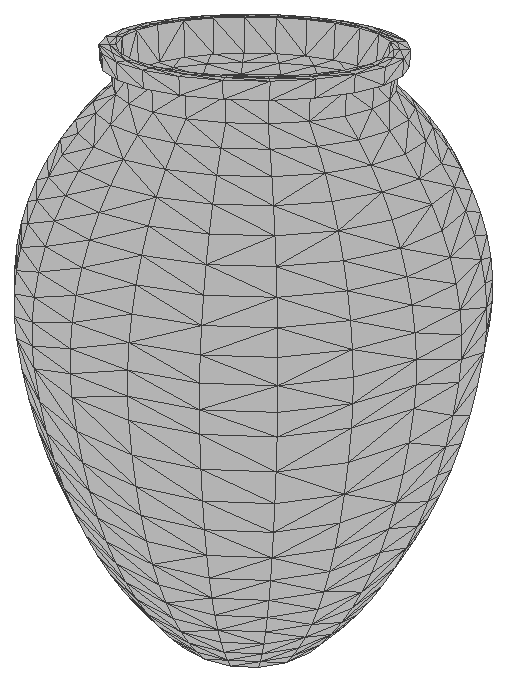
\includegraphics[width=0.2\columnwidth]{figures/vase_2}
		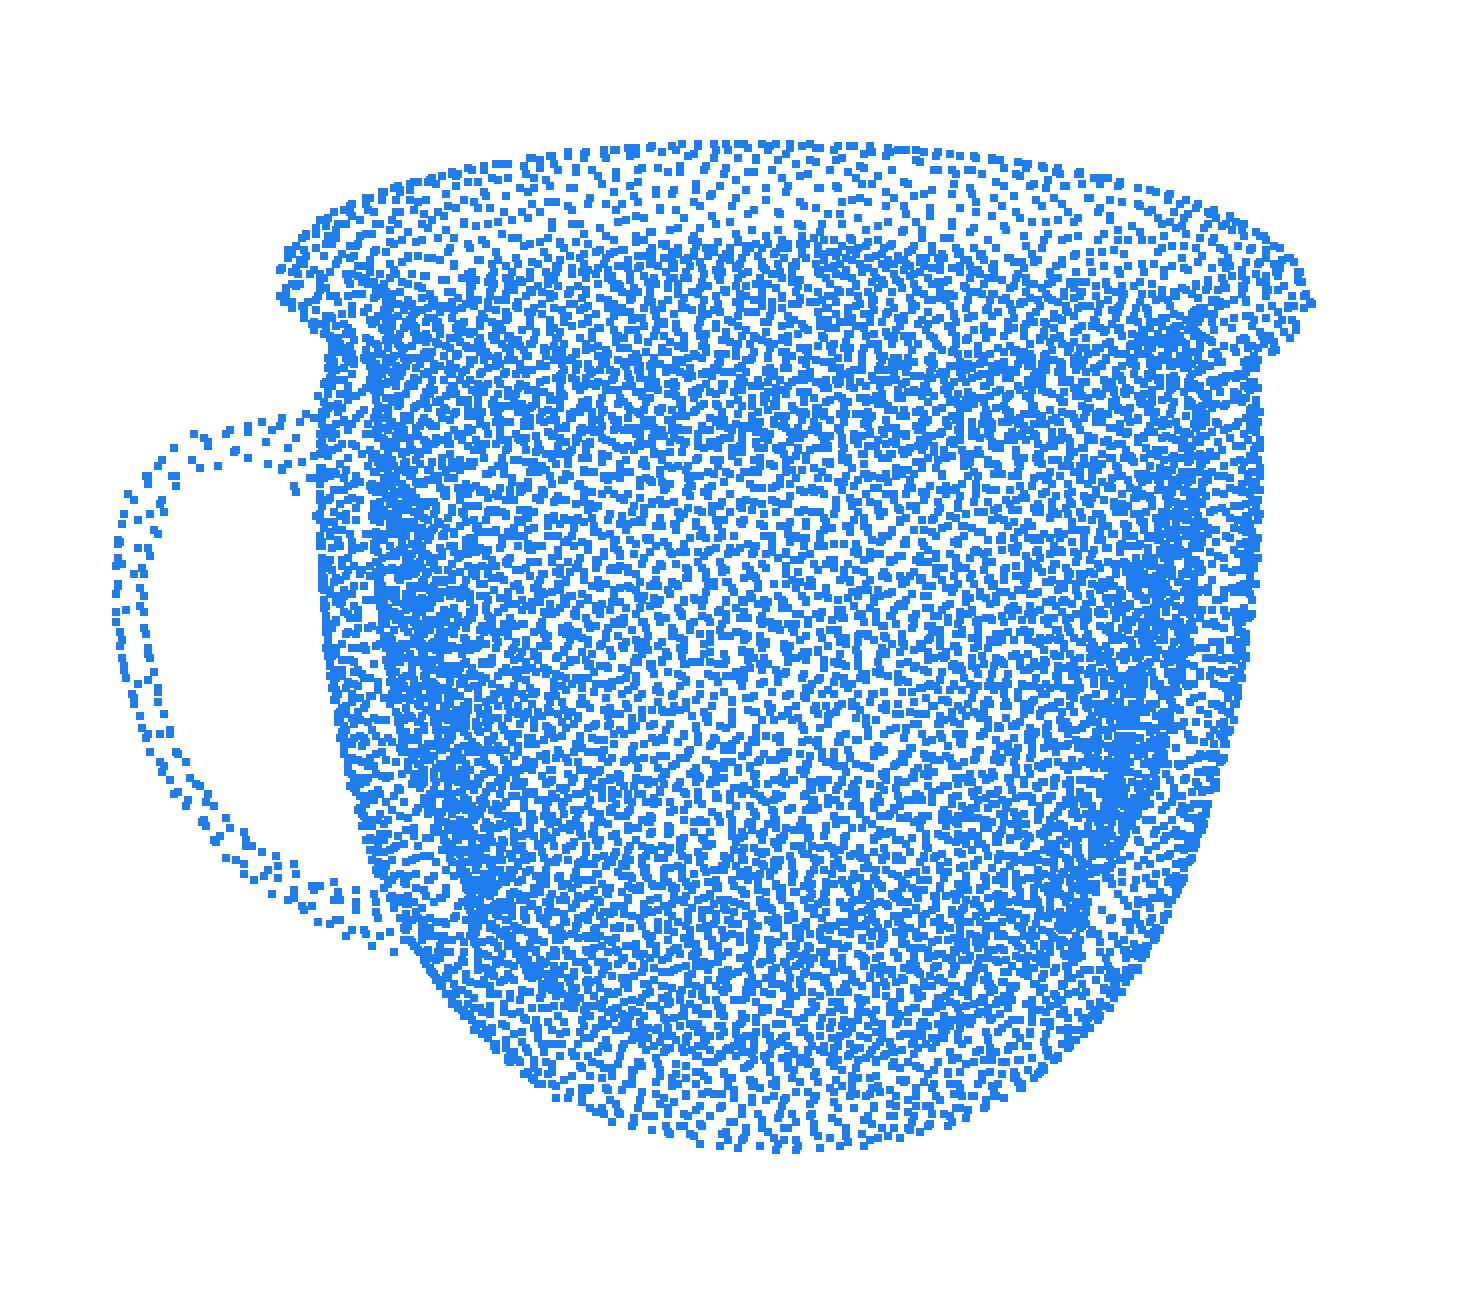
\includegraphics[width=0.3\columnwidth]{figures/cup}
		\end{figure}
		
		
	\item{\textbf{Scanned with an RGB-D camera} - multiple frames registered with PCL KinFu.}
		\begin{figure}[h]
		\centering
		
\includegraphics[width=0.3\columnwidth]{figures/kinfu_1}
		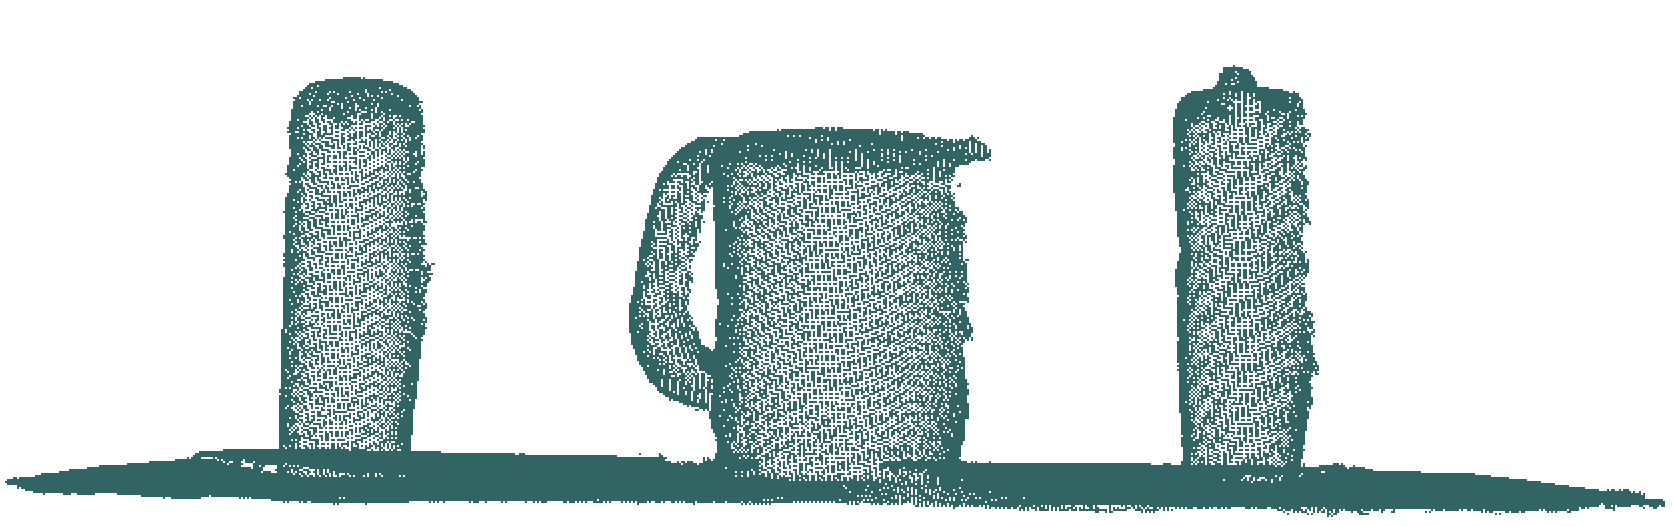
\includegraphics[width=0.3\columnwidth]{figures/kinfu_2}
		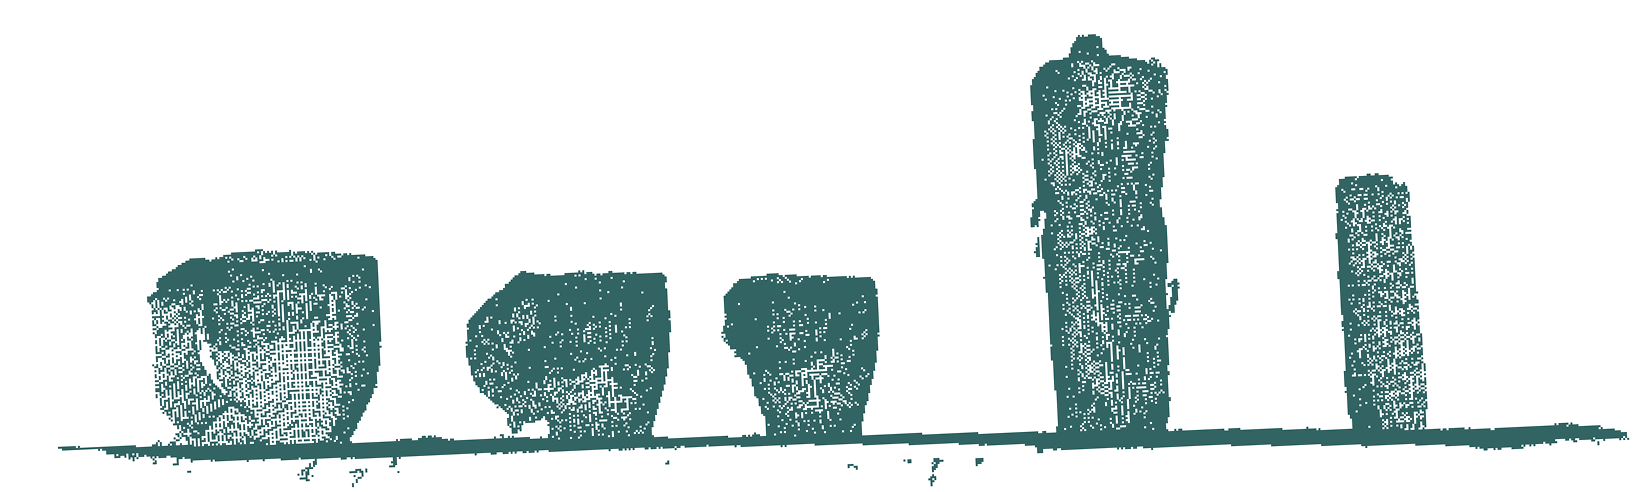
\includegraphics[width=0.3\columnwidth]{figures/kinfu_3}
		\end{figure}
\end{itemize}
		
		
		
	


%%%%%%%%%%%%%%%%%%%%%%%%%%%%%%%%%%%%%%%%%%%%%%%%%%%%%%%%%%%%
%%%%%%%%%%%%%%%%%%%%%%%%%%%%%%%%%%%%%%%%%%%%%%%%%%%%%%%%%%%%
\section {Sampling}
\label{sec:sampling}

\subsection {VTK}

\subsection {Explicit}

\subsection {Smart}


%%%%%%%%%%%%%%%%%%%%%%%%%%%%%%%%%%%%%%%%%%%%%%%%%%%%%%%%%%%%
%%%%%%%%%%%%%%%%%%%%%%%%%%%%%%%%%%%%%%%%%%%%%%%%%%%%%%%%%%%%
\section {Fitting}
\label{sec:fitting}

Various error functions with paper references

solvers: Eigen LM unstable, CERES

Derivatives - explicit (from Maple - in superquadric\_formulas.h), numerical differentiation, autodiff from CERES with Jet types + explain what Jet is

Initialisation from PCA

\subsection {Multipart Fitting with a Split \& Merge Approach}

explain what it is, reference paper

results




\section {Detection}
\label{sec:detection}

reference paper, explain how it works roughly

\subsection {Rigid Registration}

\subsection {Voting Scheme}


\section {Tabletop Demo}
\label{sec:tabletop_demo}

kinfu, kinect, figures

how I do the segmentation + clustering


\section {Conclusion and Future Work}
\label{sec:conclusion}

check Google doc

implement everything in PCL

tutorial on the website


\bibliography{references}
\bibliographystyle{plain}


\end{document}